\documentclass[11pt,letterpaper]{article}
\usepackage[T1]{fontenc}
\usepackage[utf8]{inputenc}
\usepackage{lmodern,microtype}
\usepackage[margin=0.93in,footskip=0.43in]{geometry}
\usepackage{amsmath,amssymb,booktabs,tabularx,graphicx}
\usepackage{xcolor}
\definecolor{linkink}{HTML}{155B73}
\usepackage[colorlinks=true,linkcolor=linkink,citecolor=linkink,urlcolor=linkink,pdfencoding=auto]{hyperref}
\urlstyle{same}
\setlength{\emergencystretch}{1.6em}
\setlength{\parindent}{1.25em}
\raggedbottom
\hypersetup{pdfauthor={Mohammad Ali Seyed Mahmoud},pdftitle={Request Ordering Under a Waiting Limit for LLM Prefix Reuse: A Trace Replay Study}}
\title{Request Ordering Under a Waiting Limit for LLM Prefix Reuse: A Trace Replay Study}
\author{Mohammad Ali Seyed Mahmoud\\[3pt] {\normalsize Georgia Institute of Technology}\\[-1pt] {\small\href{mailto:m.seyedmahmoud@gatech.edu}{\nolinkurl{m.seyedmahmoud@gatech.edu}}}}
\date{\small November 12, 2026\enspace\textperiodcentered\enspace This paper is licensed under \href{https://creativecommons.org/licenses/by/4.0/}{CC BY 4.0}.}
\begin{document}
\maketitle


\begin{abstract}

Can the waiting queue identify when changing request order saves enough prefill work to matter? We tested this question in a CPU replay with an LRU prefix cache and a bound on added start delay relative to first-come-first-served (FCFS). We fitted the decision rule on two Mooncake traces, fixed its predictions, then scored 3,000 held-out FreeInference requests at 36 combinations of utilization, queue depth and cache capacity. With a 500 ms waiting allowance, no configuration met the prespecified 3\% modeled prefill saving through ordering alone. The best tested LRU schedule saved at most 1.323\% over FCFS. Nine cells met the mixed criterion when the offline reference could also change eviction, all at the smallest capacity. A rule that flagged every cell had 25\% precision against an 80\% requirement. On one matched order, changing only eviction saved another 7.174 percentage points of FCFS work. An independent audit checked 540,000 request starts and found no waiting-limit violation. The result distinguishes an offline eviction opportunity from a measured ordering gain. It does not establish an optimality bound or a production latency result.

\end{abstract}

\section{What can changing the order buy?}
A prefix cache can save work if two prompts reuse the same tokens before the corresponding cache blocks are evicted. Serving a waiting request earlier might preserve that reuse; it also makes other requests wait. A useful question for a serving team is whether queue and cache statistics can identify occasions when this trade is worthwhile.

Two decisions are easy to confound in such an experiment: which request runs next, and which blocks the cache retains. RadixAttention in SGLang illustrates how a serving engine can exploit shared prefixes~\cite{sglang}. Dexter et al.\ study query ordering with prefix reuse and latency constraints and introduce \(k\)-LPM~\cite{dexter}. Liu, Yu and Yang study eviction policies on production traces, including the FreeInference data used here~\cite{fancy}. Our question is narrower: under a fixed LRU admission model and a specified waiting guard, how much modeled prefill work do the tested \emph{orders} save? We keep eviction unchanged for that comparison and report the effect of relaxing it separately. The experiment is a CPU trace replay; no SGLang server was timed.

\section{Traces, cache and service model}
\textbf{Workloads and split.} The two development traces used to fit the predictor were Mooncake conversation and tool/agent traffic~\cite{moon}. Qwen/Bailian chat and API were secondary checks; they did not select a parameter or fit a prediction rule~\cite{qwen}. Prefix identity in Qwen was reconstructed within a documented chat lineage. The selected API requests had separate lineages, preventing cross-request reuse under this model.

Before scoring, we pinned an independent FreeInference coding/assistant traffic object by revision and SHA-256~\cite{free}. Its records were stored in completion order. We read the full 327,548-record object, selected the first 5,000 by arrival time (source ordinal breaks ties), and preserved predecessor and session order. Within a user namespace we combined 32 successive 16-token blocks into a 512-token edge, interning it together with the preceding prefix. Packed future-access fields were ignored by the online rules. For every trace, the first 2,000 arrivals sized and warmed the cache under FCFS; the following 3,000 were measured without a reset. The measured holdout covers 4.47 hours of original arrivals. Different grid settings reuse these same 3,000 requests.

\textbf{Cache and pressure.} Requests are charged for missing blocks against the cache at entry. Each eligible prefix path is then admitted as a unit and protected during that admission. LRU evicts old unprotected leaves; prefixes remain closed under ancestry. Eligible paths contain at most 128 complete 512-token blocks and cannot exceed physical cache capacity. The compulsory final token and all positions outside the reusable path are charged even on a hit. The working set is the median count of distinct eligible prefix blocks across the 1,001 sliding windows of 1,000 warm-up requests. We fixed capacity at 10, 25, 50 or 100 percent of that estimate. On FreeInference these settings retain 402, 1,005, 2,010 or 4,020 blocks.

\textbf{Service and waiting.} A single nonpreemptive prefill stream processes successive chunks of up to 4,096 uncached tokens for one request. There is no inter-request batching, decoding or network time. With original context length \(L\) and \(U\) uncached positions, the modeled service cost in milliseconds is
\[
       s(U,L)=a+bU+cUL,\qquad
       (a,b,c)=(5.30609,\;0.0130596,\;1.00860\times10^{-6}).
\]
The coefficients were frozen from a nonnegative fit to cold, batch-one matrix and attention timings in NVIDIA's SGLang H100 SXM component tables, with BF16 Qwen3-8B dimensions and 36 layers~\cite{nvidia,model}. The intercept is charged once per request. We rescale interarrival gaps at each capacity to give FCFS offered utilization \(0.60,0.80\) or \(0.95\); every policy in a cell receives the same arrivals. Ready-queue caps of 4, 16 or 64 give \(3\times3\times4=36\) configurations at each waiting limit. For request \(i\), the primary constraint is
\[
       t_i^{\rm start}\le t_i^{\rm FCFS\,start}+W,\qquad W=500\ {\rm ms}.
\]
A two-second limit is a prespecified sensitivity. This is a bound on \emph{extra start delay}. Modeled time to first token (TTFT) is prefill completion minus scaled arrival; the waiting constraint does not bound its absolute value.

\section{Comparisons and decision rule}
At dispatch the scheduler takes up to the cap from already-arrived requests and commits that group; it does not wait for future arrivals to fill it. Later arrivals enter at the next group. We compare FCFS, longest resident prefix (LPM), an oldest-request/\(k\)-LPM rule adapted from Dexter et al., and a deterministic depth-first traversal of the ready prefix trie. All respect predecessor order. The \(k\)-LPM rule chooses the oldest request first and once every \(k\) picks within a group. Development compared \(k=2\) and \(4\); the prespecified tie rule selected \(2\).

The shared waiting guard checks proposed starts and the potential cost of returning to FCFS after the group. For a baseline resident block, its first subsequent hit is safe if it survives in the proposed cache and all blocks ahead of it were also ahead of it under FCFS. Let \(B_{\rm bad}\) count baseline blocks that fail this test. Once touched in a common suffix, a block's rank no longer depends on the starting state. The guard therefore reserves up to \(512 B_{\rm bad}(b+cL_{\max})\) ms for future extra misses, in addition to any positive finish-time debt. \(L_{\max}\) is one trace-level service envelope, available to every policy; the online rules do not see later individual requests. If any proposed start is late or the debt exceeds \(W\), the scheduler falls back to FCFS from its actual cache; the last group needs no suffix reserve. This is a sufficient guard. A veto does not establish that an order was infeasible.

Let \(F\) be FCFS total modeled service and \(E\) the lowest service among the feasible existing policies over a complete episode. \(R_L\) is the better of \(E\) and a feasible lookahead heuristic that uses a 16-request future rollout with eviction kept at LRU. \(R\) additionally considers changing retention using future next-use information: it protects the current path, evicts eligible leaves and verifies the resulting starts. The reference can retain the LRU fallback. Finally \(I\) uses an infinite cache on the \emph{same winning order as \(R\)}, with the same warm contents, path horizon and compulsory tail. All gaps use \(F\) as their denominator:
\[
 G_1=(F-E)/F,\quad G_{2,\mathrm{order}}=(E-R_L)/F,\quad
 G_{2,\mathrm{mixed}}=(E-R)/F,\quad G_3=(R-I)/F .
\]
\(G_1\) and \(G_{2,\mathrm{order}}\) isolate gains achieved through ordering. \(G_{2,\mathrm{mixed}}\) allows a different eviction policy. \(G_3\) is a fixed-order residual; the reference is a feasible heuristic, not an optimizer. The residual is not a universal capacity penalty.

We registered a cell as material for ordering if either \(G_1\) or \(G_{2,\mathrm{order}}\) reached 3\%, the achieving policy had no waiting violation, and its p99 modeled TTFT was at most 110\% of FCFS. We also evaluated the analogous mixed criterion, substituting \(G_{2,\mathrm{mixed}}\). In development we fitted a single-threshold rule (including constant predictions) over four quantities obtained by observing FCFS: fraction of ready block occurrences shared across requests, capacity ratio, median reuse distance divided by capacity, and mean visible queue depth. We saved the fitted rules and the holdout flags before computing held-out policy scores. The decision to proceed required at least one correct positive flag and precision of at least 80\% among flags at the primary \(W\). A rule predicting no positives cannot pass. The grid cells are not independent replicates.

\section{Results}
No primary FreeInference configuration achieved the registered materiality threshold with eviction held at LRU. The best complete LRU trajectory tested saved at most 1.323\% over FCFS. The maxima of individual gaps in Table~\ref{tab:gaps} occur in different cells and cannot be added. Extending the waiting allowance to two seconds did not yield a material ordering cell. Figure~\ref{fig:gaps} shows why a conclusion based only on the mixed reference would differ.

\begin{table}[htbp]\centering\small
\caption{Maximum held-out gap as a percentage of FCFS modeled prefill service. Counts apply to the full combined materiality test, including TTFT and waiting.}\label{tab:gaps}\par\vspace{4pt}
\begin{tabular}{@{}lrr@{}}\toprule
Quantity & 500 ms (primary) & 2 s (sensitivity)\\\midrule
Existing order vs.\ FCFS, \(G_1\) & 1.261\% & 1.344\%\\
Further gain with LRU fixed, \(G_{2,\mathrm{order}}\) & 0.591\% & 0.699\%\\
Further gain allowing eviction, \(G_{2,\mathrm{mixed}}\) & 7.765\% & 7.626\%\\
Residual to infinite cache, \(G_3\) & 9.989\% & 9.978\%\\
Material cells: ordering only & 0/36 & 0/36\\
Material cells: mixed comparison & 9/36 & 9/36\\\bottomrule
\end{tabular}\end{table}

\begin{figure}[htbp]\centering
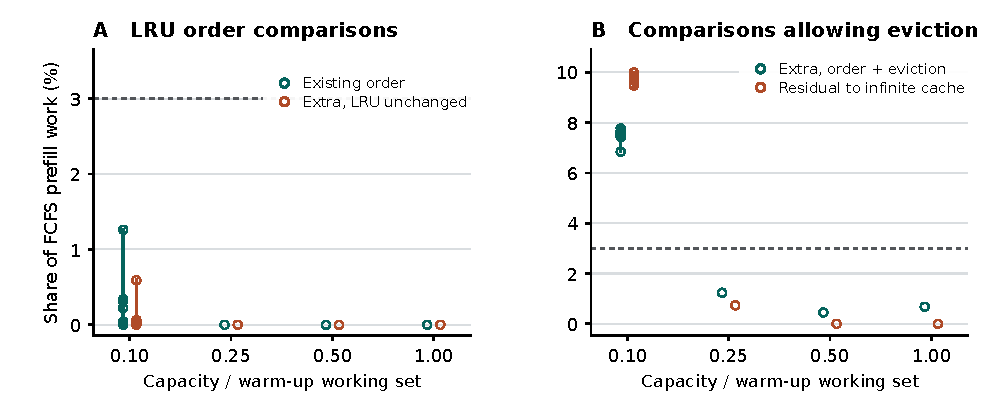
\includegraphics[width=\linewidth]{heldout.pdf}
\caption{Recorded work gaps in the 36 primary FreeInference configurations. Each capacity has nine utilization/queue-cap combinations. Points can coincide; vertical lines span the observed range. The dashed line marks 3\% of FCFS work, the work component of the materiality rule. The panels use different vertical scales to show the small LRU gains.}\label{fig:gaps}
\end{figure}

All nine mixed positives occurred at 402 blocks, where mixed savings ranged from 6.846 to 7.765\%. One comparison isolates eviction on a matched order. At utilization 0.60 and queue cap 16, future-informed ordering under LRU saved 0.591 percentage points beyond the best existing order. Changing only eviction \emph{on that same order} saved another 7.174 points. This attributes the larger saving in this cell to offline eviction; it does not identify an online rule that would attain it.

\textbf{Did the queues fill?} Every configured ready cap was reached in each corresponding primary cell. At cap 64, mean ready depth was 21.5--43.7. Across primary LPM, selected \(k\)-LPM and DFS trajectories, the guard accepted 3,063 of 9,220 proposed group reorderings and vetoed 6,157. These counts include multiple replays of the same traffic. Across the 180 primary LRU trajectories, the worst added start delay was 499.092 ms. An independent ordered-dictionary reconstruction of saved schedules checked all 540,000 measured starts with no waiting-limit, ready-cap, group-membership or precedence violations. It also reproduced token work, step counts and TTFT quantiles.

\textbf{Did the predictor transfer?} Neither primary Mooncake development trace had a material LRU ordering cell (0/72 combined); all 72 passed the mixed criterion. The fitted rules thus flagged no cells for ordering and every cell for the mixed comparison. The secondary Qwen traces also had no ordering positives; under the mixed criterion chat had 36/36 and API 0/36. On FreeInference, ordering-only precision was undefined (no flags). The mixed rule had nine true and 27 false positives, for 25\% precision and 9/9 recall. The smallest-capacity association was discovered on this holdout and is not a validated predictor. Neither decision rule authorized GPU validation.

\section{Interpretation and limits}
The 3\% target was not attained by these guarded LRU orderings on the measured period. A different guard could admit other legal schedules; the feasible lookahead is not a proof that no order can do better. The study also cannot estimate a population frequency from 36 configurations of one traffic period. User namespacing, discrete prefix blocks, one service stream and the finite prefix horizon restrict what the replay captures.

Absolute latency is particularly uncertain. On the primary grid, modeled FCFS median TTFT ranged from 10.5 to 319.5 seconds, and p99 from 37.0 to 44.3 minutes. Even on reserved cold calibration points the fit differed by up to 13.2\%. Of the 3,000 measured prompts, 2,304 exceeded the longest calibrated point (16,384 tokens), and 1,855 exceeded the model configuration's standard 40,960-token context. No end-to-end or cached-extension latency was validated. At 72 MiB per 512-token block under the modeled BF16 configuration, the four retained pools alone represent 28.3, 70.7, 141.3 and 282.7 GiB, before weights or workspace. The larger pools are virtual pressure settings. These results justify stopping this particular ordering pilot before GPU validation; they do not establish a production TTFT improvement, a limit for all possible orderings, or the performance of an online eviction policy.

\section*{Artifact and attribution}
The FreeInference trace was released by Yiyu Liu, Minlan Yu and Juncheng Yang under \href{https://creativecommons.org/licenses/by/4.0/}{CC BY 4.0}. The artifact documents the chronological selection, user namespacing, block aggregation and truncation applied here. It also records the original development/test split and the order of prediction and scoring. No request text is required.


\noindent\textbf{Code and data.} The simulator, protocol, fitted rules, time-stamped predictions, per-policy results, figure source and audit witnesses and instructions for reproducing the results are available in the \href{https://github.com/smahmoud66/prefix-cache-studies/blob/7a2f9a970a0bb851a5517bf48c3c95dd73cb538b/docs/ordering.md}{public GitHub artifact} (revision \href{https://github.com/smahmoud66/prefix-cache-studies/commit/7a2f9a970a0bb851a5517bf48c3c95dd73cb538b}{\texttt{7a2f9a970a}}). Repository: \url{https://github.com/smahmoud66/prefix-cache-studies}.

\noindent\textbf{Tool use.} OpenAI Codex assisted with preparing the manuscript and computational artifact and with running the release checks. The reported measurements come from the archived pilot.

\begin{thebibliography}{99}

\bibitem{sglang} L. Zheng et al. \href{https://proceedings.nips.cc/paper_files/paper/2024/hash/724be4472168f31ba1c9ac630f15dec8-Abstract-Conference.html}{SGLang: Efficient Execution of Structured Language Model Programs}. NeurIPS, 2024.

\bibitem{dexter} Dexter et al. \href{https://proceedings.neurips.cc/paper_files/paper/2025/hash/878bbdf6227315995c207561211ddb53-Abstract-Conference.html}{LLM Query Scheduling with Prefix Reuse and Latency Constraints}. NeurIPS, 2025.

\bibitem{fancy} Y. Liu, M. Yu and J. Yang. \href{https://arxiv.org/abs/2609.28870v3}{When Fancy Eviction Fails: Rethinking Cache Replacement for LLM Prefix Reuse}. arXiv:2609.28870v3, 2026.

\bibitem{moon} Mooncake trace authors. \href{https://github.com/kvcache-ai/Mooncake/tree/3cca71daccf2a7afb8fe3f0295358f70e3a69fdb/FAST25-release/traces}{Mooncake FAST 2025 release: production conversation and tool/agent traces}. Dataset, revision 3cca71d.

\bibitem{qwen} Qwen/Bailian trace authors. \href{https://github.com/alibaba-edu/qwen-bailian-usagetraces-anon/tree/5f7439c51ec248a0c585f7d90a41a6f57773b912}{Qwen/Bailian anonymized usage traces}. Dataset, revision 5f7439c.

\bibitem{free} Y. Liu, M. Yu and J. Yang. \href{https://huggingface.co/datasets/harvardMadsys/2026_prefixcache/tree/ba89a343a048073dda72617bb6087910da6214d0}{LLM Prefix-Cache Block Traces: FreeInference}. Dataset, revision ba89a34, 2026.

\bibitem{nvidia} NVIDIA AIConfigurator contributors. \href{https://github.com/ai-dynamo/aiconfigurator/tree/6cd6f9686ab7de6e8fb28171d6e350ee0aa4ed39/aic-core/src/aiconfigurator_core/systems/data/h100_sxm}{H100 SXM component performance tables: SGLang 0.5.14}. Software and measurements, revision 6cd6f96.

\bibitem{model} Qwen team. \href{https://huggingface.co/Qwen/Qwen3-8B/blob/b968826d9c46dd6066d109eabc6255188de91218/config.json}{Qwen3-8B model configuration}. Model card and configuration, revision b968826.

\end{thebibliography}

\end{document}
